\begin{frame}[fragile]{}
	\frametitle{IBM Implementation: Qiskit}
	\framesubtitle{Backend \& Quantum Registers}
	\vspace*{0.5cm}
		\begin{adjustbox}{max width=0.8\textwidth}
			\begin{python}
				
from qiskit import *
from qiskit import QuantumCircuit
from qiskit.circuit.quantumcircuit import QuantumCircuit
from qiskit.visualization import plot_histogram

backend = BasicAer.get_backend('qasm_simulator')
#backend = BasicAer.get_backend('statevector_simulator')

'''Quantum register
https://quantumcomputing.stackexchange.com/questions/4907/
qiskit-is-there-any-way-to-discard-the-results-of-a-measurement'''

q = QuantumRegister(2, 'q')
a = QuantumRegister(1, 'a')
c = ClassicalRegister(2, 'c')
			\end{python}
		\end{adjustbox}

\end{frame}

\begin{frame}[fragile]{}
	\frametitle{IBM Implementation: Qiskit}
	\framesubtitle{Quantum Circuit}
	\vspace*{0.25cm}
	\begin{adjustbox}{max width=0.7\textwidth}
		\begin{python}
#Circuit
circ = QuantumCircuit(q,a,c) # type: qiskit.circuit.quantumcircuit.QuantumCircuit

# ===== prepare the states: psi^{[0]} =====
circ.iden(q[0])
circ.iden(q[1])
circ.x(a[0])

#===== Initialization: psi^{[1]} =====
circ.h(q[0])
circ.h(q[1])
circ.h(a[0])
circ.barrier(q)

#===== Sign flip: psi^{[2]} =====
circ.x(q[0])
circ.ccx(q[0], q[1], a[0])
circ.x(q[0])

circ.barrier(q)

#===== Inversion about average: psi^{[3]} =====
circ.h(q[0])
circ.h(q[1])
circ.x(q[0])
circ.x(q[1])

circ.cz(q[0], q[1])

circ.x(q[0])
circ.x(q[1])
		\end{python}
	\end{adjustbox}
	
\end{frame}

\begin{frame}[fragile]{}
	\frametitle{IBM Implementation: Qiskit}
	\framesubtitle{Measurement}
	\vspace*{0.25cm}
	\begin{adjustbox}{max width=0.6\textwidth}
		\begin{python}
#===== Meaurement =====
circ.measure(q,c)

#job
job = execute(circ, backend=backend, shots=1600)
result = job.result()

#circuit
figure = circ.draw(output='mpl')
figure.savefig('../data/images/qiskit-circuit.png')

#histogram
counts = result.get_counts(circ)
print("Total counts:")
print(counts)

figure = plot_histogram(counts)
figure.savefig('../data/images/qiskit-histogram.png')
		\end{python}
	\end{adjustbox}
	
\end{frame}

\begin{frame}[fragile]{}
	\frametitle{IBM Implementation: Qiskit}
	\framesubtitle{Measurement}
	\begin{columns}
		\begin{column}{0.75\textwidth}
			\begin{figure}
				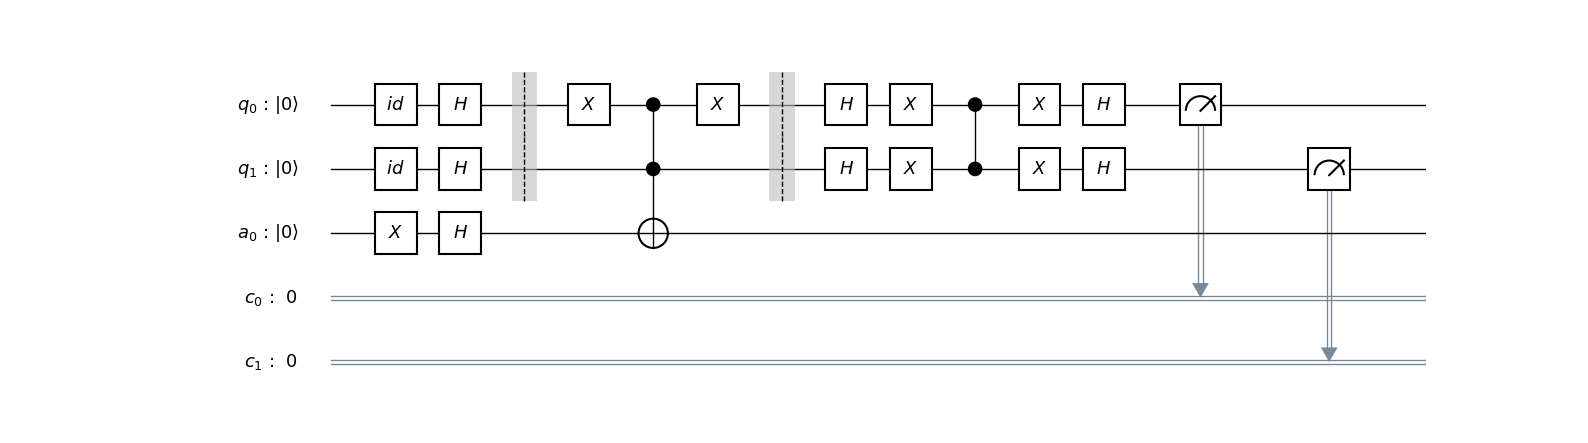
\includegraphics[trim=190 0 190 0,width=0.9\textwidth]{code/data/images/qiskit-circuit.png}
				\caption{Quantum Circuit}
			\end{figure}
		\end{column}
		\begin{column}{0.25\textwidth}  %%<--- here
			\begin{figure}
				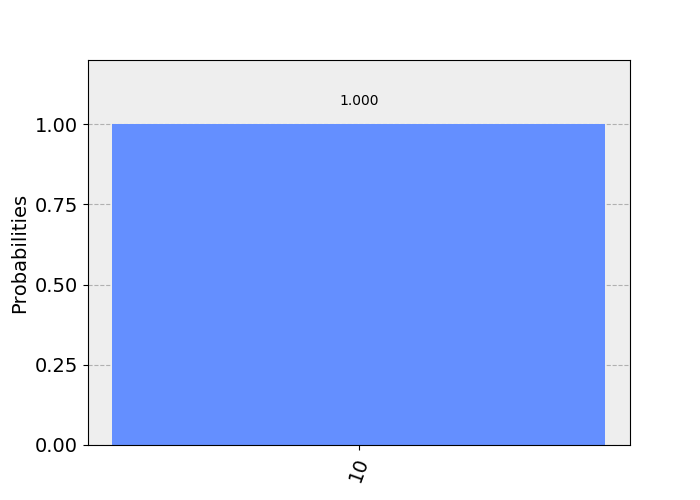
\includegraphics[width=\textwidth]{code/data/images/qiskit-histogram.png}
				\caption{Histogram}
			\end{figure}
		\end{column}
	\end{columns}
\end{frame}	

\begin{frame}[fragile]{}
	\frametitle{IBM Implementation: Quantum Experience}
	\framesubtitle{\href{https://www.research.ibm.com/ibm-q/technology/experience/}{https://www.research.ibm.com/ibm-q/technology/experience/}}
	\begin{columns}
		\begin{column}{0.75\textwidth}
			\begin{figure}
				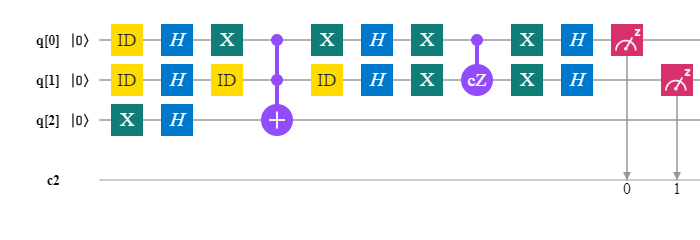
\includegraphics[trim=0 0 0 0,width=0.9\textwidth]{figures/ibm-implementation/circuit.png}
				\caption{Quantum Circuit}
			\end{figure}
		\end{column}
		\begin{column}{0.25\textwidth}  %%<--- here
			\begin{figure}
				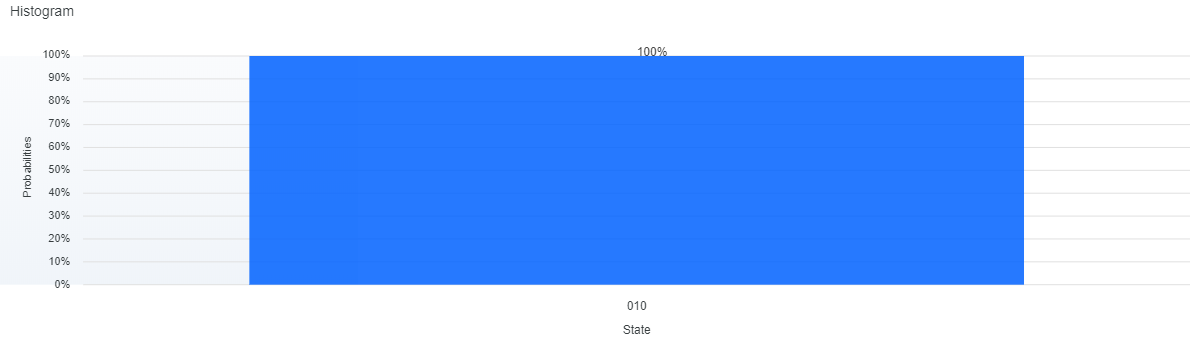
\includegraphics[width=\textwidth]{figures/ibm-implementation/histogram.png}
				\caption{Histogram}
			\end{figure}
		\end{column}
	\end{columns}
\end{frame}	